\documentclass[10pt]{article}

\pagestyle{empty}

\setlength{\textheight}{250mm}
\setlength{\textwidth}{180mm}
\setlength{\oddsidemargin}{-8mm}
\setlength{\topmargin}{-1.5cm}

\usepackage{amsmath}
\usepackage{amsthm}
\usepackage{psfrag}
\usepackage{graphicx}
\usepackage{bm}
\usepackage{mathrsfs}
\usepackage{icomma} % pacchetto per limitare lo spazio standard posto dopo la virgola in caso che la virgola sia tra cifre
\usepackage{amsfonts} % amplia i caratteri matematici disponibili
\usepackage{amssymb}
%\usepackage{wrapfig}
\usepackage{empheq}

\usepackage{epstopdf}
\usepackage[utf8x]{inputenc}
\usepackage{ifthen}

\usepackage[italian]{babel}
%\usepackage[latin1]{inputenc}

%\include{def}

%\newcommand{\kg}{\textrm{kg}}
%\newcommand{\K}{\textrm{K}}
%\newcommand{\m} {\textrm{m}}
%\newcommand{\dm}{\textrm{dm}}
%\newcommand{\cm}{\textrm{cm}}
%\newcommand{\mm}{\textrm{mm}}
%\newcommand{\s} {\textrm{s}}
%\newcommand{\N} {\textrm{N}}
%\renewcommand{\Pa}{\textrm{Pa}}
%\newtheorem{exerciseS}{Esercizio}
\def \flagSect{0} % 1    : numerazione
		  % else : niente
%\newcommand{\taitol}[1]  % stile titolo
%{
%%{\textit{#1}}
%{#1}
%}
\def \soluzione{Soluzione}
\def \partePrima{Concetti. }
\def \parteSeconda{Svolgimento. }
%\def \parteTerza{}
\newcommand{\sol}{\subsubsection*{\soluzione}}
\newcommand{\partone}{\ \ \ \ \ \textbf{\partePrima}}
\newcommand{\parttwo}{\vspace{0.2cm}\textbf{\parteSeconda}}

\ifnum\flagSect=1
\newtheorem{esercizio}{Esercizio}%[section]
\else
\newtheorem*{esercizio}{Esercizio}
\fi

\newtheorem*{teorema}{Teorema}
\newtheorem*{lemma}{Lemma}

% ###########################################################
%\def \flagSect{0} % 1    : numerazione
		  % else : niente
%\newcommand{\taitol}[1]  % stile titolo
%{
%%{\textit{#1}}
%{#1}
%}
\def \soluzione{Soluzione}
\def \partePrima{Concetti. }
\def \parteSeconda{Svolgimento. }
%\def \parteTerza{}
\newcommand{\sol}{\subsubsection*{\soluzione}}
\newcommand{\partone}{\ \ \ \ \ \textbf{\partePrima}}
\newcommand{\parttwo}{\vspace{0.2cm}\textbf{\parteSeconda}}

\ifnum\flagSect=1
\newtheorem{esercizio}{Esercizio}%[section]
\else
\newtheorem*{esercizio}{Esercizio}
\fi

\newtheorem*{teorema}{Teorema}
\newtheorem*{lemma}{Lemma}

% ###########################################################
%\def \flagSect{0} % 1    : numerazione
		  % else : niente
%\newcommand{\taitol}[1]  % stile titolo
%{
%%{\textit{#1}}
%{#1}
%}
\def \soluzione{Soluzione}
\def \partePrima{Concetti. }
\def \parteSeconda{Svolgimento. }
%\def \parteTerza{}
\newcommand{\sol}{\subsubsection*{\soluzione}}
\newcommand{\partone}{\ \ \ \ \ \textbf{\partePrima}}
\newcommand{\parttwo}{\vspace{0.2cm}\textbf{\parteSeconda}}

\ifnum\flagSect=1
\newtheorem{esercizio}{Esercizio}%[section]
\else
\newtheorem*{esercizio}{Esercizio}
\fi

\newtheorem*{teorema}{Teorema}
\newtheorem*{lemma}{Lemma}

% ###########################################################
%\input{logicNumb}
%\newcommand{\sectionIf}[2]
%{
%   \ifthenelse{\equal{#1}{1}}
%              {\subsection{#2}}{\subsection*{#2}}
%}
% ###########################################################

%\newcommand{\sectionIf}[2]
%{
%   \ifthenelse{\equal{#1}{1}}
%              {\subsection{#2}}{\subsection*{#2}}
%}
% ###########################################################

%\newcommand{\sectionIf}[2]
%{
%   \ifthenelse{\equal{#1}{1}}
%              {\subsection{#2}}{\subsection*{#2}}
%}
% ###########################################################



\begin{document}

\begin{center}
\textbf{Esercizi per il corso di Fluidodinamica} 
\medskip
\end{center}



%%%%%%%%%%%%%%%%%%%%%%%%%%%%%%%%%%%%%%%%%%%%%%%%%%%%%%%%%%%%%%%%%%

%%%%%%%%%%%%%%%%%%%%%%%%%%%%%%%%%%%%%%%%%%%%%%%%%%%%%%%%%%%%%%%%%%

%%%%%%%%%%%%%%%%%%%%%%%%%%%%%%%%%%%%%%%%%%%%%%%%%%%%%%%%%%%%%%%%%%
\noindent
\begin{tabular}{cc}
\begin{minipage}[b]{0.60\textwidth}
\begin{exerciseS}[Corrente in un canale piano - Newton-Poiseuille]
In un canale piano, di lunghezza e apertura infinita, 
orizzontale, di altezza $H=1.51\ mm$,
delimitato da una parete inferiore fissa e da una parete superiore 
mobile con velocit\`a orizzontale, costante e positiva $U=0.31\ m/s$.
scorre acqua in condizioni standard.
Per quale valore del gradiente di pressione $G_P = -\partial P/\partial x$ la portata nel canale risulta nulla? \newline
Si trascurino le forze di volume.

\vspace{0.5cm}
($ Re = 441$, $G_p = - 930\  Pa/m$)
\end{exerciseS}
\end{minipage}
&
\begin{minipage}[b]{0.35\textwidth}
   \begin{center}
   \includegraphics[width=0.90\textwidth,trim = 160 350 200 320]{./fig/slnEsatte-newton-couette}
   \end{center}
\end{minipage}
\end{tabular}

\sol

\partone
 Semplificazione delle equazioni di NS in coordinate cartesiane per descrivere la corrente in un canale piano infinito messo in moto da un gradiente di pressione (corrente di Poiseuille) e dal trascinamento dovuto al movimento di una parete del canale (corrente di Newton).

\parttwo
In questo problema, la corrente nel canale ha due "forzanti": il moto a (velocità costante) della parete superiore e il gradiente di pressione $G_P$ lungo il canale. Il problema chiede di trovare il valore di $G_P$ tale che la portata nel canale sia nulla quando i due effetti si combinano.
Il problema viene risolto ricavando il profilo di velocità in funzione del gradiente di velocità dalle equazioni di NS opportunamente semplificate e successivamente il valore del gradiente di pressione necessario ad avere portata nulla. La geometria del problema suggerisce di utilizzare un sistema di coordinate cartesiane.

\begin{itemize}

  \item Scrittura delle equazioni di NS in coordinate cartesiane in 2 dimensioni.
%  
 \begin{equation}
\begin{cases}
  \dfrac{\partial u}{\partial t} + u \dfrac{\partial u}{\partial x}
  + v \dfrac{\partial u}{\partial y} - \nu \left( 
  \dfrac{\partial^2 u}{\partial x^2} +
  \dfrac{\partial^2 u}{\partial y^2} \right)
  + \dfrac{1}{\rho} \dfrac{\partial p}{\partial x} = f_x \\
  \dfrac{\partial v}{\partial t} + u \dfrac{\partial v}{\partial x}
  + v \dfrac{\partial v}{\partial y} - \nu \left( 
  \dfrac{\partial^2 v}{\partial x^2} +
  \dfrac{\partial^2 v}{\partial y^2} \right)
  + \dfrac{1}{\rho} \dfrac{\partial p}{\partial y} = f_y \\
  \dfrac{\partial u}{\partial x} + \dfrac{\partial v}{\partial y} = 0
\end{cases}
\end{equation}

  \item Semplificazione delle equazioni di NS per il problema considerato. Vengono fatte le seguenti ipotesi:
\begin{itemize}
\item problema stazionario: $\dfrac{\partial}{\partial t} = 0$;
\item direzione $x$ omogenea (canale infinito in direzione $x$): $\dfrac{\partial u}{\partial x} = \dfrac{\partial v}{\partial x} = 0$; 
\begin{remark}
non si può dire altrettanto della pressione, a causa del ruolo che questa ha nelle equazioni di NS incomprimibili. Il campo di pressione può essere interpretato come un moltiplicatore di Lagrange necessario a imporre il vincolo di incomprimibilità. Inoltre, ad eccezione di alcune condizioni al contorno, non appare mai direttamente come pressione $p$ ma solamente con le sue derivate spaziali. Da un punto di vista più fisico, la differenza di pressione lungo il canale è la forzante che mette in moto il fluido in una corrente di Poiseuille.
\end{remark}
\item la condizione $\dfrac{\partial u}{\partial x} = 0$ inserita nel vincolo di incomprimibilità, implica $\dfrac{\partial v}{\partial y}=0$; poichè $\dfrac{\partial v}{\partial x}=\dfrac{\partial v}{\partial y}=0$ segue che $v = \text{cost} = 0$, poiché è nulla a parete per la condizione al contorno di adesione, $\bm{u} = \bm{0}$.
\item no forze di volume: $\bm{f} = 0$.
\end{itemize}
%
Le equazioni di NS possono essere semplificate
\begin{equation}
\begin{cases}
  \nu \dfrac{\partial^2 u}{\partial y^2} = \dfrac{\partial p}{\partial x} \\
  \dfrac{\partial p}{\partial y} = 0  
\end{cases}
\end{equation}

Dalla seconda segue che la pressione può essere funzione solo di $x$. Nella prima, il termine a sinistra dell'uguale è funzione solo di $y$; quello di destra
può essere funzione solo di x: l'uguaglianza implica che entrambi i membri sono 
costanti. Definiamo questa costante come $ G_P = - \dfrac{\partial p}{\partial x} $: si noti che questo è il "gradiente di pressione" lungo il canale, cambiato di segno.
%  \begin{equation}
%  \end{equation}
%  
  \begin{equation}
  \begin{cases}
    - \mu u''(y) = G_P & y \in[0,H] \\
    u(0) = 0  \\ u(H) = U
  \end{cases}
  \end{equation}
  
  
  
  \item Soluzione dell'equazione differenziale  con dati al contorno: si integra due volte e si impongono le condizioni al contorno per ottenere la componente $u$ del campo di velocità.
  \begin{equation}
    \Rightarrow u(y) = -\dfrac{G_P}{2 \mu} y^2 + \left( \dfrac{G_P}{2 \mu}H
    + \dfrac{U}{H} \right) y \ .
  \end{equation}
  
  \item Calcolo della portata come integrale della velocità. 
  \begin{equation}
    Q = \int_{0}^{H} u(y) dy = \dfrac{G_P}{12 \mu} H^3 + \dfrac{1}{2} U H
  \end{equation}
  %
  Infine, imponendo la condizione di portata nulla $Q=0$, si ottiene il valore di $G_P$:
  \begin{equation}
    G_P = -6\dfrac{\mu U}{H^2} \qquad \Rightarrow \qquad G_P = - 930 Pa/m
  \end{equation}
  
\end{itemize}



%%%%%%%%%%%%%%%%%%%%%%%%%%%%%%%%%%%%%%%%%%%%%%%%%%%%%%%%%%%%%%%%%%

%%%%%%%%%%%%%%%%%%%%%%%%%%%%%%%%%%%%%%%%%%%%%%%%%%%%%%%%%%%%%%%%%%
%%%%%%%%%%%%%%%%%%%%%%%%%%%%%%%%%%%%%%%%%%%%%%%%%%%%%%%%%%%%%%%%%%

\end{document}
